\documentclass{article}
\usepackage[margin=1in]{geometry}
\usepackage{amsmath,amsthm,amssymb}
\usepackage{bbm,enumerate,mathtools}
\usepackage{tikz,pgfplots}
\usepackage{chessboard}
\usepackage[hidelinks]{hyperref}
\usepackage{multicol} % Problem 35

\newenvironment{question}{\begin{trivlist}\item[\textbf{Question.}]}{\end{trivlist}}
\newenvironment{note}{\begin{trivlist}\item[\textbf{Note.}]}{\end{trivlist}}
\newenvironment{references}{\begin{trivlist}\item[\textbf{References.}]}{\end{trivlist}}
\newenvironment{related}{\begin{trivlist}\item[\textbf{Related.}]\end{trivlist}\begin{enumerate}}{\end{enumerate}}


\begin{document}
\rating{4}{4}
Consider a peaceable queens problem in an $n \times n \times n$ chess
``cube'', where a queen can move in any diagonal direction.
\begin{figure}[ht!]
  \centering
  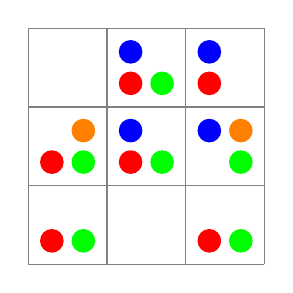
\begin{tikzpicture}
    \draw [gray] (0,0) grid (3, 3);
    \node at (0.5, 2.5) {\Huge \textcolor{red}{\symqueen}};
    \node at (1.5, 0.5) {\Huge \textcolor{black!20!green}{\symqueen}};
    \foreach \x/\y/\c in {
      0.3/0.3/red, 0.3/1.3/red, 1.3/1.3/red, 1.3/2.3/red, 2.3/0.3/red, 2.3/2.3/red,
      0.7/0.3/green, 0.7/1.3/green, 1.7/1.3/green, 1.7/2.3/green, 2.7/0.3/green, 2.7/1.3/green,
      1.3/1.7/blue, 1.3/2.7/blue, 2.3/1.7/blue, 2.3/2.7/blue,
      0.7/1.7/orange, 2.7/1.7/orange}
    {
      \fill[\c] (\x, \y) circle (0.15cm);
    }
  \end{tikzpicture}\hspace{0.5cm}
  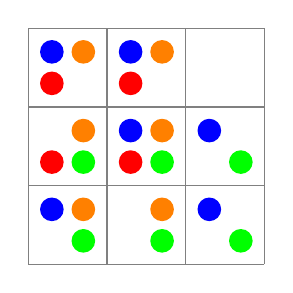
\begin{tikzpicture}
    \draw [gray] (0,0) grid (3, 3);
    \node at (2.5, 2.5) {\Huge \textcolor{blue}{\symqueen}};
    \foreach \x/\y/\c in {
      0.3/1.3/red, 0.3/2.3/red, 1.3/1.3/red, 1.3/2.3/red,
      0.7/0.3/green, 0.7/1.3/green, 1.7/0.3/green, 1.7/1.3/green, 2.7/0.3/green, 2.7/1.3/green,
      0.3/0.7/blue, 0.3/2.7/blue, 1.3/1.7/blue, 1.3/2.7/blue, 2.3/0.7/blue, 2.3/1.7/blue,
      0.7/0.7/orange, 0.7/1.7/orange, 0.7/2.7/orange, 1.7/0.7/orange, 1.7/1.7/orange, 1.7/2.7/orange}
    {
      \fill[\c] (\x, \y) circle (0.15cm);
    }
  \end{tikzpicture}\hspace{0.5cm}
  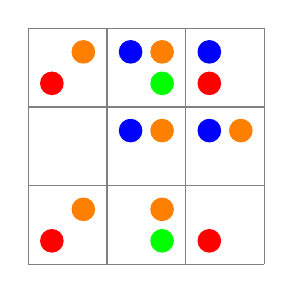
\begin{tikzpicture}
    \draw [gray] (0,0) grid (3, 3);
    \node at (0.5, 1.5) {\Huge \textcolor{orange}{\symqueen}};
    \foreach \x/\y/\c in {
      0.3/0.3/red, 0.3/2.3/red, 2.3/0.3/red, 2.3/2.3/red,
      1.7/0.3/green, 1.7/2.3/green,
      1.3/1.7/blue, 1.3/2.7/blue, 2.3/1.7/blue, 2.3/2.7/blue,
      0.7/0.7/orange, 0.7/2.7/orange, 1.7/0.7/orange, 1.7/1.7/orange, 1.7/2.7/orange, 2.7/1.7/orange}
    {
      \fill[\c] (\x, \y) circle (0.15cm);
    }
  \end{tikzpicture}
  \caption{
    At least four hyper-queens can be placed peaceably on a
    $3 \times 3 \times 3$ board.
  }
\end{figure}
\begin{question}
  What is the greatest number of queens that can be placed on an
  $n \times n \times n$ board?
\end{question}

\begin{related}
  \item If $n^{k-1}$ queens can be placed on a
    $\displaystyle\underbrace{n \times n \times \hdots \times n}_{k}$ board
    for sufficently large $n$, how large must $n$ be?
\end{related}
\begin{references}
  \item \url{https://math.stackexchange.com/q/2232287/121988}
\end{references}
\end{document}
